\begin{figure}[tb]
  \begin{subfigure}{\columnwidth}
    \centering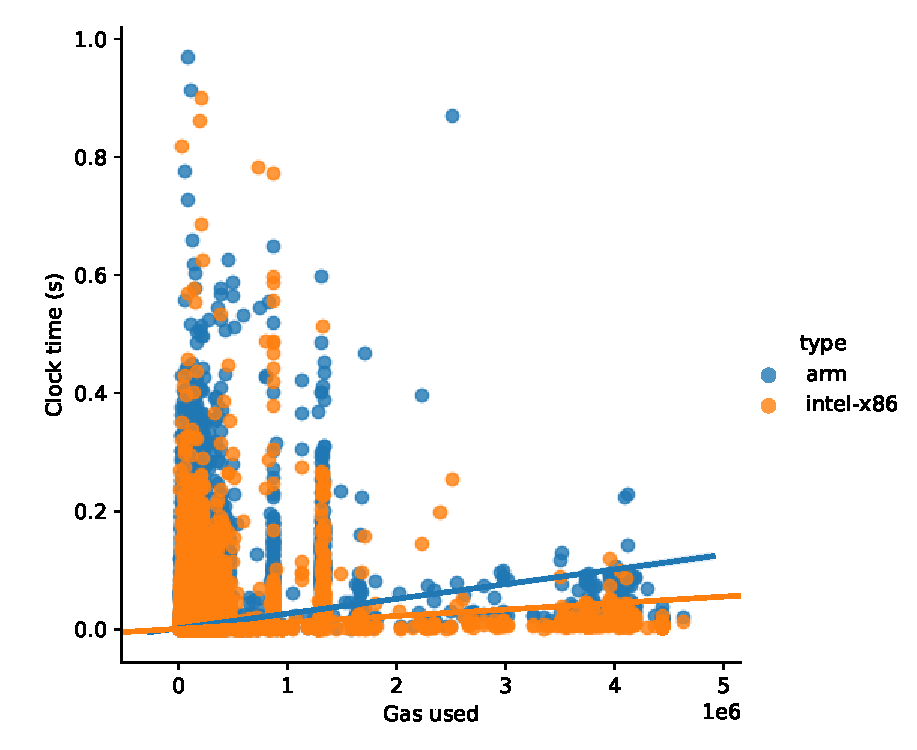
\includegraphics[width=\columnwidth]{3-evm-security/figures/cpu-gas-x86-arm-1500000-2000000.pdf}
    \caption{Relation between clock time and gas used.}
    \label{fig:x86-arm-cpu}
  \end{subfigure}

  \begin{subfigure}{\columnwidth}
    \centering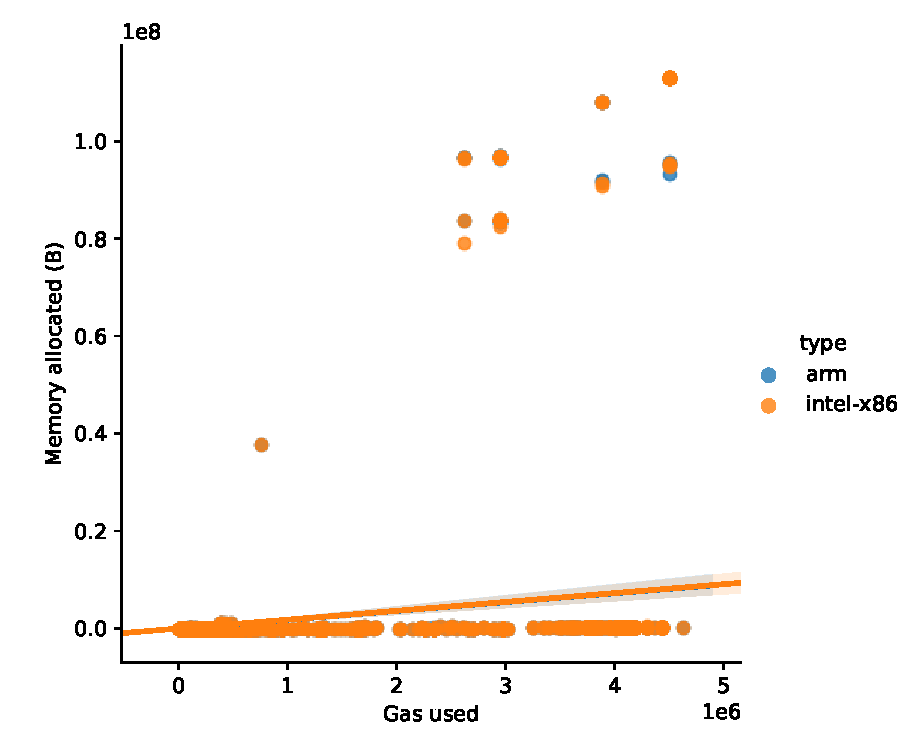
\includegraphics[width=\columnwidth]{3-evm-security/figures/memory-gas-x86-arm-1500000-2000000.pdf}
    \caption{Relation between memory allocated and gas used.}
    \label{fig:x86-arm-memory}
  \end{subfigure}

  \caption{Resource usage comparison between x86 and ARM.}
  \label{fig:x86-arm}
\end{figure}

\section{Comparison Across Platforms}
\label{sec:cloud}

\subsection{x86 vs. ARM}

\begin{itemize}
\item ARM: Cortex-A72
\item X86: Intel(R) Xeon(R) Platinum 8124M
\end{itemize}

In \autoref{fig:x86-arm-cpu}, we show the relation between gas usage and CPU clock time for both x86 and ARM. We can see that the memory allocated is exactly the same on both platforms but that the clock time is in general higher on ARM than on x86.

\subsection{Linux vs. Windows}
Same gas, CPU cycles, maybe memory

\subsection{VM-based vs. Bare Metal}
Proportionate slowdown--are

\subsection{Cloud-based vs. Local Machine}
Metering built into cloud platforms, correlation, etc.

\subsection{Summary}
